\documentclass[12pt]{article}

\title{Group Homework 9}
\author{G2 - Robert Krency, Austin Pringle, Anthony Stepich}
\date{\today}

\usepackage{tikz}
\usepackage{amsmath}
\usepackage{graphicx}
\usepackage{tabularx}
\usepackage{multicol}
\usepackage{enumitem}

\usepackage[normalem]{ulem}

% Geometry 
\usepackage{geometry}
\geometry{letterpaper, left=1in, top=1in, right=1in, bottom=1in}

% Macros
\newcommand{\definition}[1]{\underline{\textbf{#1}}}

\newcommand{\encircle}[1]{%
  \tikz[baseline=(X.base)] 
    \node (X) [draw, shape=circle, inner sep=0] {\strut #1};}

\renewcommand{\arraystretch}{1.5}

% Begin Document
\begin{document}

\maketitle

\pagebreak

\begin{enumerate}

    %1
    \item Minimal State Diagram with output of 1 when sequences 1010 or 1101 are detected; overlapping allowed.
    \vspace{5mm}

    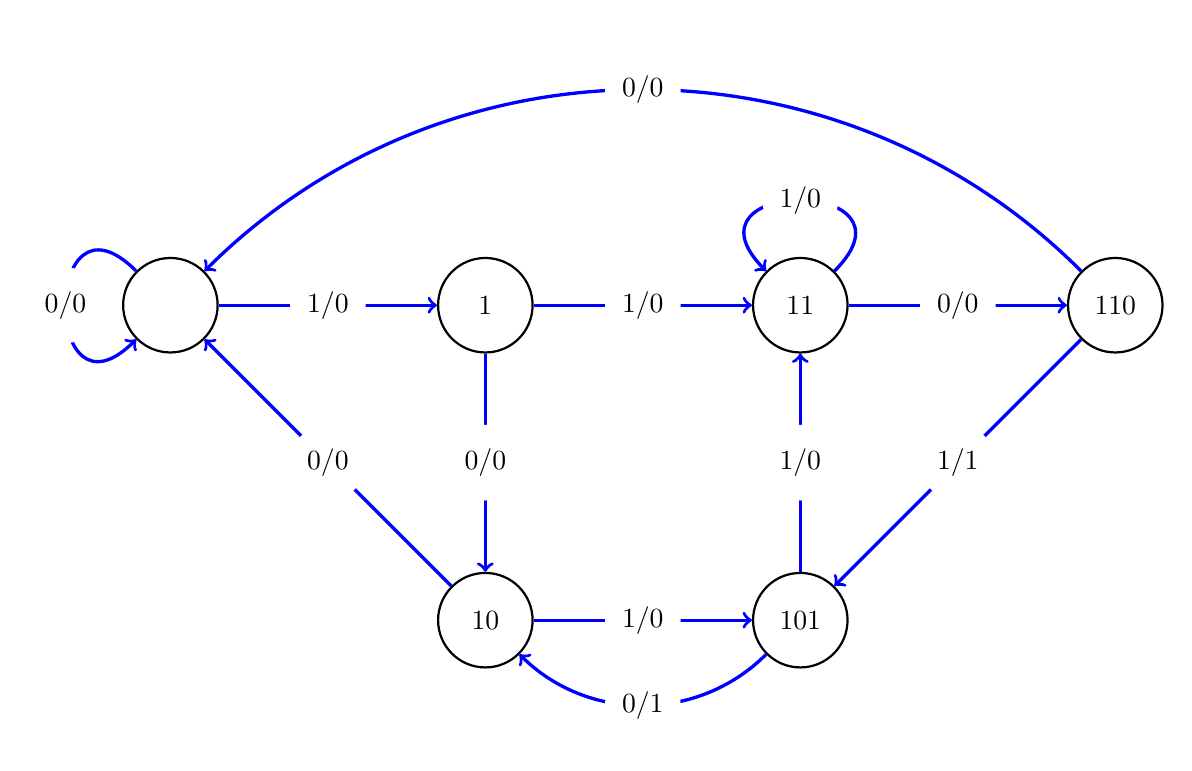
\begin{tikzpicture}
        
        \begin{scope}[every node/.style={circle,thick,draw,minimum size=12mm}]
            \node (1) at (0,0) {};
            \node (2) at (4,0) {1};
            \node (3) at (8,0) {11};
            \node (4) at (12,0) {110};
            \node (5) at (4,-4) {10};
            \node (7) at (8,-4) {101};
        \end{scope}
    
        \begin{scope}[every node/.style={fill=white,circle}, every edge/.style={draw=blue,very thick}]
            \path [->] (1) edge node {1/0} (2);
            \path [->] (1) edge [out=135,in=225,looseness=5] node {0/0} (1);

            \path [->] (2) edge node {1/0} (3);
            \path [->] (2) edge node {0/0} (5);

            \path [->] (3) edge [out=45,in=135,looseness=5] node {1/0} (3);
            \path [->] (3) edge node {0/0} (4);

            \path [->] (4) edge [out=135,in=45] node {0/0} (1);
            \path [->] (4) edge node {1/1} (7);

            \path [->] (5) edge node {1/0} (7);
            \path [->] (5) edge node {0/0} (1);

            \path [->] (7) edge node {1/0} (3);
            \path [->] (7) edge [out=225,in=315] node {0/1} (5);
        \end{scope}

    \end{tikzpicture}

    %2
    \item Minimal State Table for the above sequence detector, beginning with state A. \\ \\

    \begin{tabular}{ >{\centering}p{0.2\textwidth} p{0.2\textwidth} p{0.2\textwidth}}

          & $X=0$ & $X=1$ \\ 
        P  & NS,z & NS,z  \\ \hline

        A  & A,0  & B,0  \\
        B  & EH,0 & C,0  \\
        C  & D,0  & C,0  \\
        D  & A,0  & FG,1 \\
        EH & A,0  & FG,0 \\
        FG & EH,1 & C,0  \\

    \end{tabular}

    \pagebreak

    %3
    \item Transition Table \\ \\

    \begin{tabular}{ l l l l | l l l l | l l l l}

         &  & $X=0$ & $X=1$ & $X$ & $=$ & $0$ & & $X$ & $=$ & $0$ \\ 
        P & abc  & NS,z & NS,z & Ja & Ka & Jb & Kb & Ja & Ka & Jb & Kb \\ \hline

        A  & 000 & 000,0 & 001,0 \\
        B  & 001 & 100,0 & 010,0 \\
        C  & 010 & 011,0 & 010,0 \\
        D  & 011 & 000,0 & 101,1 \\
        EH & 100 & 000,0 & 101,0 \\
        FG & 101 & 100,1 & 010,0 \\
           & 110 & xxx,x & xxx,x \\
           & 111 & xxx,x & xxx,x 

    \end{tabular}

    \vspace{2cm}


\end{enumerate}

\end{document}